\documentclass[a4paper,10pt]{article}
\usepackage[utf8x]{inputenc}
\usepackage{amsmath}
\usepackage{graphicx}
\usepackage[english]{babel}
\usepackage{url}
\usepackage{epstopdf}
\usepackage{subfig}
\usepackage{graphicx}

\title{Procesamiento Avanzado de Imágenes\\IEE3784}
\author{\textbf{Tarea 01}\\Norman F. Sáez\\nfsaez@uc.cl}
\date{\today}

\begin{document}
\maketitle
\section{Pregunta 1}
Se utiliza el algoritmo de Cox de Boor para calcular tanto las bases como
b-splines, de acuerdo a los puntos de control entregados en la tarea y el
vector de nodos.  Se considera que en cada iteración, se hacen 5 sumas y  2
multiplicaciones por coordenada ``x'', de esta manera, para 100 puntos un resultado de
144 sumas por coordenada ``x'' y 60 multiplicaciones por
coordenada ``x''. El total por coordenada es de \textbf{\textit{288
sumas}} y \textbf{\textit{120 multiplicaciones}}, por cada \textbf{100 puntos}.
El total de la curva de 400 puntos es de 1152 sumas y de 480 multiplicaciones.

\begin{figure}[ht!]
  \centering
  \subfloat[B-Splines: Puntos de control en azul]{\label{fig:img1a}\includegraphics[width=0.50\textwidth]{img/img1a.eps}}
  ~ 
  \subfloat[Bases $B_{4,1}=rojo$, $B_{4,2}=verde$, $B_{4,3}=azul$, $B_{4,4}=magenta$]{\label{fig:img1b}\includegraphics[width=0.50\textwidth]{img/img1b.eps}}
  ~ 
  \caption{B-Splines y Bases}
  \label{fig:p1}
\end{figure}
Cabe mencionar que solo se debe evaluar donde todas las bases tienen valor, no en todos los nodos. ver figura \ref{fig:p1}

\section{Pregunta 2}
Para cada punto se evaluó en $f(t,t,t)=F(t)$, utilizando el algoritmo visto en
clases. Para calcular, se define primero: $r_1 < r_2 < r_3 < s_1 < s_2 < s_3$.
De esta manera, los puntos de control vienen a ser; $f(r_1,r_2,r_3)$,
$f(r_1,r_2,s_1)$, $f(r_1,s_1,s_2)$ y $f(s_1,s_2,s_3)$, para la primera iteración. Luego encontramos:
De esta manera se tiene:
$$f(r_1,r_2,r_3) = P_1$$
$$f(r_1,r_2,s_1) = P_2$$
$$f(r_1,s_1,s_2) = P_3$$
$$f(s_1,s_2,s_3) = P_4$$

$r$ y $s$ de simular forma ($K$ vector de nodos entregado como dato):
$$r_1 = K_1$$
$$r_2 = K_2$$
$$r_3 = K_3$$

$$s_1 = K_4$$
$$s_2 = K_5$$
$$s_3 = K_6$$

Ahora para la primera iteracion obtenemos lo siguiente:
$$f(r_1,r_2,t) = ((s_1 - t)/(s_1-r_3))*f(r_1,r_2,r_3) + ((t - r_3)/(s_1 - r_3))*f(r_1,r_2,s_1)$$
$$f(r_1,s_1,t) = ((s_2 - t)/(s_2-r_2))*f(r_1,r_2,s_1) + ((t - r_2)/(s_2 - r_2))*f(r_1,s_1,s_2)$$
$$f(s_1,s_2,t) = ((s_3 - t)/(s_3-r_1))*f(r_1,s_1,s_2) + ((t - r_1)/(s_3 - r_1))*f(s_1,s_2,s_3)$$

De los valores anteriores se puede obtener ahora los ulimos dos puntos intermedios:
$$f(r_1,t_1,t) = ((s_1 - t)/(s_1-r_2))*f(r_1,r_2,t) + ((t - r_2)/(s_1 - r_2))*f(r_1,s_1,t)$$
$$f(s_1,t_1,t) = ((s_2 - t)/(s_2-r_1))*f(r_1,s_1,t) + ((t - r_1)/(s_2 - r_1))*f(s_1,s_2,t)$$

Para finalmente terminar en la tercera iteracion obteniendo $F(t)=f(t,t,t)$ deseado:
$$f(t,t,t) = ((s_1 - t)/(s_1-r_1))*f(r_1,t_1,t) + ((t - r_1)/(s_1 - r_1))*f(s_1,t_1,t)$$

Sin embargo los resultados no son los esperados y se pueden ver en \ref{fig:p2}
\begin{figure}[ht!]
  \centering
  \subfloat[B-Spline Forma Polar: Puntos de control en azul]{\label{fig:img2}\includegraphics[width=0.80\textwidth]{img/img2.eps}}
  ~ 
  \caption{B-Splines calculado en forma polar}
  \label{fig:p2}
\end{figure}
Se utilizaron 4 puntos de control y luego los cuatro siguiente, con el resultado obtenido. Como se puede apreciar claramente, no es una curva continua
por lo que lo mas probable es que no este bien aplicado el metodo. Los puntos en azul son los puntos de control de la curva.

\newpage
\section{Pregunta 3}
Es necesario aplicar para esta pregunta un sistema de ecuaciones, de modo que:
$$A*X=P$$

En donde $P$ son los puntos a buscar, y la matriz $A$ sea el
resultado de una combinacion lineal entre las bases que pueden ser encontradas
( ya que se pide buscar una b-spline cubica uniforme y periodica, por ende las
bases son conocidas) y el parametro $t$ entregado como dato.
%\begin{figure}[ht!]
%  \centering
%  \subfloat[]{\label{fig:img3}\includegraphics[width=0.80\textwidth]{img/img3.eps}}
%  ~ 
%  \caption{}
%  \label{fig:p3}
%\end{figure}

\section{Pregunta 4}
Aqui se grafica con el metodo de Casteljau, una curva de Bezier. La diferencia es que no hay un vector de nodos que
controle la curva o que pondere con mayor peso uno u otro punt
Aqui se grafica con el metodo de Casteljau, una curva de Bezier. La diferencia es que no hay un vector de nodos que
controle la curva o que pondere con mayor peso uno u otro punto. ver figura \ref{fig:p4}
\begin{figure}[ht!]
  \centering
  \subfloat[B-Spline, Casteljau: Puntos de control en azul]{\label{fig:img4}\includegraphics[width=0.80\textwidth]{img/img4.eps}}
  ~ 
  \caption{B-Splines calculado usando Casteljau}
  \label{fig:p4}
\end{figure}

\end{document}
